\section{Problema biológico}

La biología, y en particular la genética, han tenido un lugar destacado en el siglo XX gracias a enormes avances como el descubrimiento de la estructura molecular del ADN, con el aporte de Franklin  \cite{FRANKLIN1953}; y Crick y Watson \cite{WATSON1953}. A partir de esos hitos científicos, se sucedieron grandes esfuerzos a nivel internacional, como el Proyecto Genoma Humano \cite{Consortium2001} o ENCODE \cite{Consortium2012}, que tienen como objetivo general el mapeo entre código genético humano y sus elementos funcionales. Estos trabajos, sumados a los recientes avances en las tecnologías de secuenciación masiva, han generado un creciente volumen de datos genómicos que a su vez favorecieron la aparición de nuevos tipos de tratamientos en el área de la medicina personalizada \cite{doi:10.1056/NEJMp1006304}. 

La medicina personalizada o de precisión es un modelo médico en donde las intervenciones se realizan a individuos o a grupos en riesgo a diferencia del modelo tradicional que apunta a la población en general. \textbf{Dentro de este área, uno de los objetivos críticos que se busca resolver es la detección de variaciones genéticas que deriven en enfermedades}.

\subsection{El dogma central de la biología}

El genoma humano está compuesto por el ADN (ácido desoxirribonucleico), que se encuentra en los 23 pares de cromosomas (moléculas de ADN) y en las mitocondrias, en las que existe una molécula de ADN denominada ADN mitocondrial. El ADN se compone de 4 bases: Adenina, Timina, Citosina, y Guanina. Estas bases se representan con su letra inicial: A, T, C y G. Cada una de estas bases está unida a otra (Adenina-Timina y Citosina-Guanina) formando pares de bases en forma helicoidal. A su vez estas cadenas pueden ser divididas en genes, que son regiones del ADN que codifican funciones. El conjunto de genes de un organismo es lo que se conoce como el genoma.

Para entender un poco cómo funciona el proceso por el cual la información genética se expresa en el organismo recurrimos al llamado "Dogma central de la biología", esbozado por Francis Crick en 1958 \cite{CRICK1958} y revisado en 1970 \cite{CRICK1970}. Este dogma, si bien fue ampliado a lo largo del tiempo, explica de forma general este proceso. Como vemos en la figura \ref{fig:esquema_dogma}, el ADN (ácido desoxirribonucleico) se transcribe en forma de ARN para luego formar una proteína. El ARN (ácido ribonucleico), es una mólecula polimérica, al igual que el ADN, y también posee las mismas bases que el ADN, excepto la timina (T) que se reemplaza por el uracilo (U). Finalmente, el ARN es utilizado para unir los aminoácidos que forman la secuencia proteica, en un proceso denominado Traducción. La secuencia del ARN se compone de tripletes adyacentes de bases que se denominan codones, y cada aminoácido está codificado por uno de estos codones (ver figura \ref{fig:table_codon}). 

\newpage

\begin{figure}[H]
\centering
    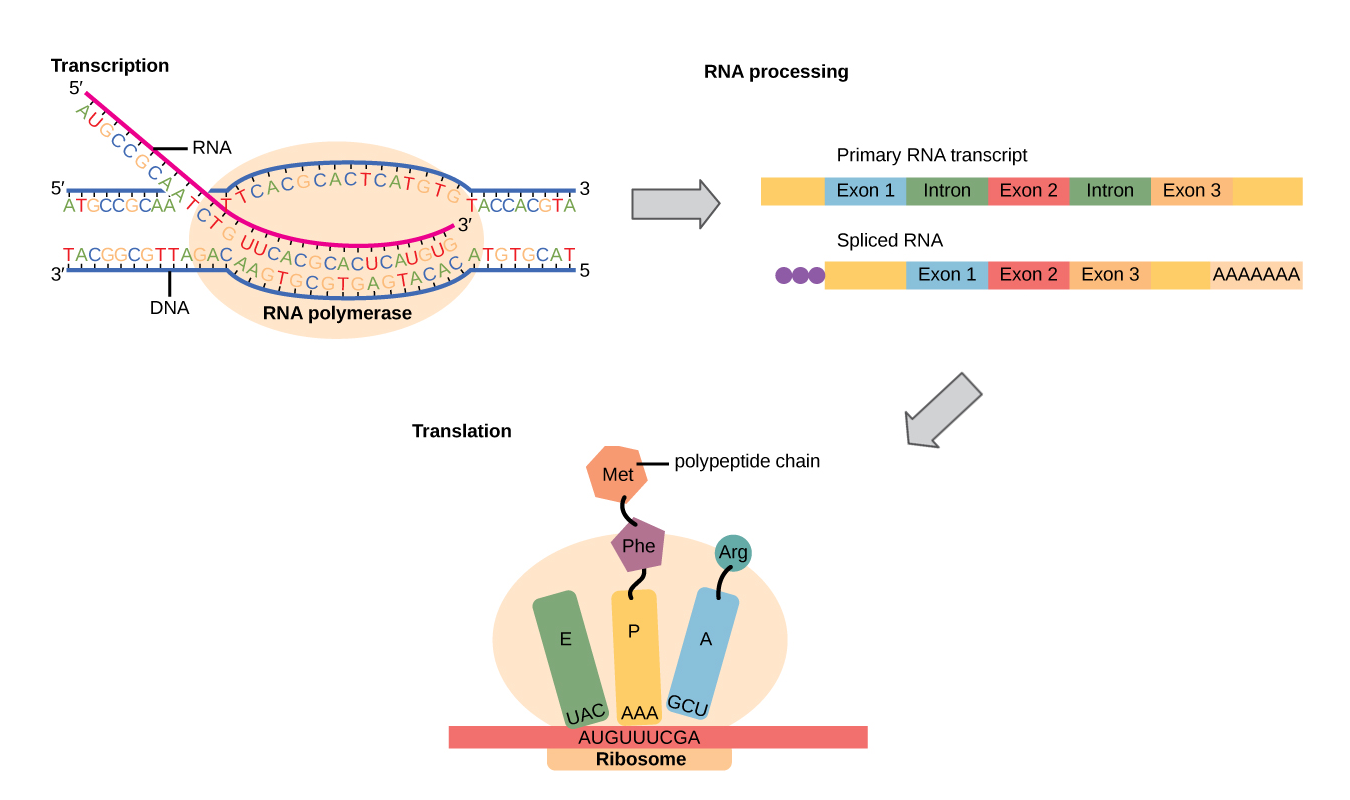
\includegraphics[width=\textwidth]{documents/latex/figures/1/dogma.png}
    \caption{Transferencia de la información genética. El ADN es transcripto en forma de ARN (ARN mensajero). Luego el ARN mensajero es ensamblado uniendo los exones (partes codificantes del gen) en un proceso denominado \textit{splicing}. Por último, los ribosomas usan la información del ARN mensajero para unir los aminoácidos en forma de proteína. Imagen tomada de OpenStax \cite{OpenStaxCNX}.}
    \label{fig:esquema_dogma}
\end{figure}

\begin{figure}[H]
\centering
    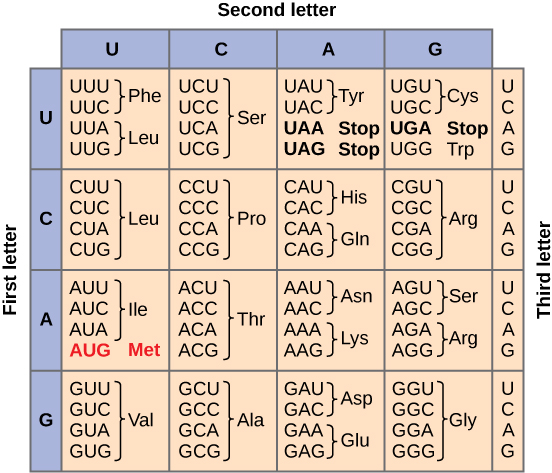
\includegraphics[scale=0.8]{documents/latex/figures/1/tableCodon.jpg}
    \caption{Tabla de codones para generar un determinado aminoácido o símbolo de terminación (\textit{Stop}). Imagen tomada de OpenStax \cite{OpenStaxCNX}.}
    \label{fig:table_codon}
\end{figure}

\newpage

\subsection{Variaciones genéticas}

Las variaciones genéticas son diferencias en el ADN entre individuos de una población \cite{EMBL}. Estas variaciones pueden ser causadas por mutaciones en el momento de la replicación del material genético, pudiendo ser de carácter permanente. Las mutaciones genéticas suelen representar un porcentaje muy pequeño con respecto a la secuencia completa del genoma (alrededor del 0.5\%), pero muchas de ellas suelen ser responsables de variaciones fenotípicas, es decir, nuestros rasgos ``observables''. 

Estas variaciones se pueden dividir en tres grupos principales:

\begin{itemize}
    \item Polimorfismos de un sólo nucleótido (SNPs): sustitución de un único par de bases. 
    \item Inserciones o deleciones (indels): pueden ocurrir en un intervalo grande del ADN de entre 2 a 200 pares de bases.
    
    \item Variaciones estructurales: ocurren en secuencias largas de bases, y pueden ser indels, inversiones, duplicaciones, entre otras.
    
\end{itemize}

Finalmente, cualquiera de estas variaciones pueden ser beneficiosas para el organismo, neutrales (sin efecto alguno) o perjudiciales. 

\subsection{Polimorfismos de un sólo nucleótido (SNPs)}

En el marco de esta tesis estudiaremos los polimorfismos de un sólo nucleótido, o SNPs por sus siglas en inglés (Single Nucleotide Polymorphism). Una persona posee en promedio alrededor de 4 a 5 millones de SNPs. Mientras la mayoría de ellos no tiene efecto en su desarrollo, algunos de ellos pueden variar la respuesta a ciertas drogas, o el riesgo de sufrir algunas enfermedades.

En la figura \ref{fig:snp_types} podemos ver los distintos tipos de SNP. De acuerdo al lugar, pueden ocurrir en una zona codificante, es decir una porción del gen que codifica una proteína, o en una zona no codificante, como los intrones (partes del gen no codificante).

Dentro de las sustituciones en la zona codificante, algunas mutaciones pueden ser sinónimas, es decir que existe un cambio en uno de los nucleótidos del ADN pero no genera un cambio en el aminoácido que codifica. Podemos ver en la tabla \ref{fig:table_codon} que muchos codones codifican el mismo aminoácido, por ejemplo, los codones AUU, AUC y AUA codifican el aminoácido isoleucina. Luego, si en la cadena de ADN, el codón AUA sufre una mutación en su último nucleótido, pasando a ser AUC, dicho codón seguirá codificando para el mismo aminoácido. Otro tipo de sustituciones, denominadas mutaciones sin sentido (\textit{nonsense}) codifican un codón de terminación (\textit{stop}), que resulta en un fin de codificación prematuro y en general una proteína no funcional.

En particular estudiaremos los SNPs con cambio de sentido (\textit{missense}), es decir aquellos que deriven en un cambio de aminoácido en la proteína producida por la variante del gen. 

\begin{figure}[H]
\centering
    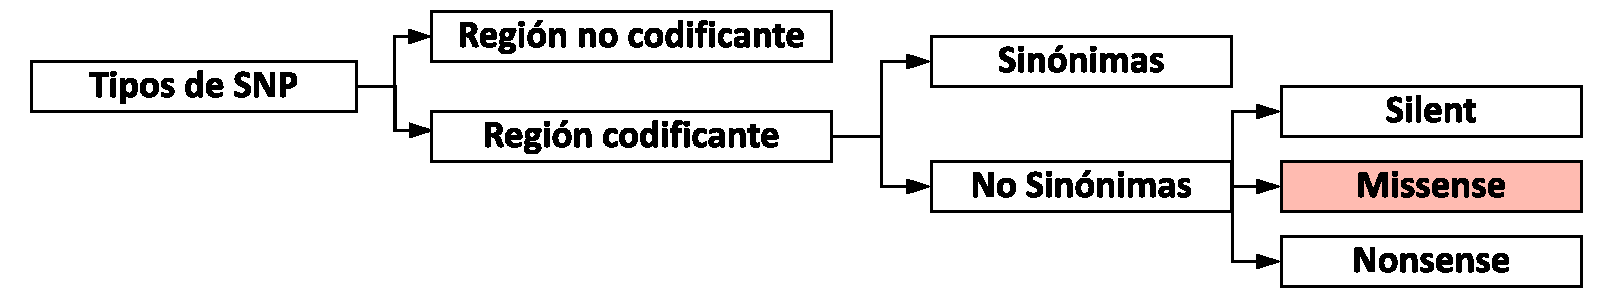
\includegraphics[scale=0.7]{documents/latex/figures/1/snp_types.pdf}
    \caption{Diferentes tipos de SNP de acuerdo a su posición en el genoma y su efecto. En este trabajo nos concentraremos únicamente en las sustituciones \textit{missense}. }
    \label{fig:snp_types}
\end{figure}

\subsection{Bases de datos \textit{ómicas}}

En la actualidad existen diferentes bases de datos públicas (dbSNP, SNPedia, HapMap, entre otras) que registran millones de estos SNPs \textit{missense}. Los costos de una secuenciación completa siguen bajando de forma acelerada desde el Proyecto Genoma Humano \cite{sequencingcost} (ver figura \ref{fig:cost_per_genome}). Esto ha permitido generar un número creciente de estudios que permiten asociar polimorfismos genéticos a enfermedades (ver figura \ref{fig:dbsnp_growth_rate}). Diferentes bases, como Humsavar \cite{humsavar} o Clinvar \cite{clinvar}, contienen reportes curados con dichos resultados, que se actualizan periódicamente y pueden variar con nueva evidencia. Sin embargo, todavía existe un gran número de SNPs \textit{missense} de los cuales se desconoce su efecto en el organismo. 

% Side by side figures 
\begin{figure}[H]
\begin{minipage}[c]{0.45\linewidth}
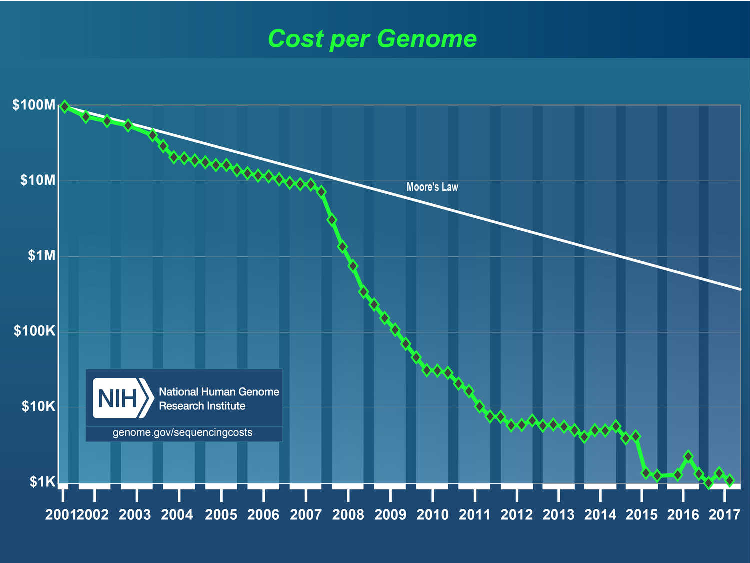
\includegraphics[width=\linewidth]{documents/latex/figures/1/costpergenome_2017.pdf}
\caption{Costo por secuenciación del genoma (NCBI-NIH, 2017). La curva verde corresponde al costo en dólares y la curva blanca equivale a la curva de la ley de Moore, es decir, si se reduciera a la mitad cada año.}
\label{fig:cost_per_genome}
\end{minipage}
\hfill
\begin{minipage}[c]{0.45\linewidth}
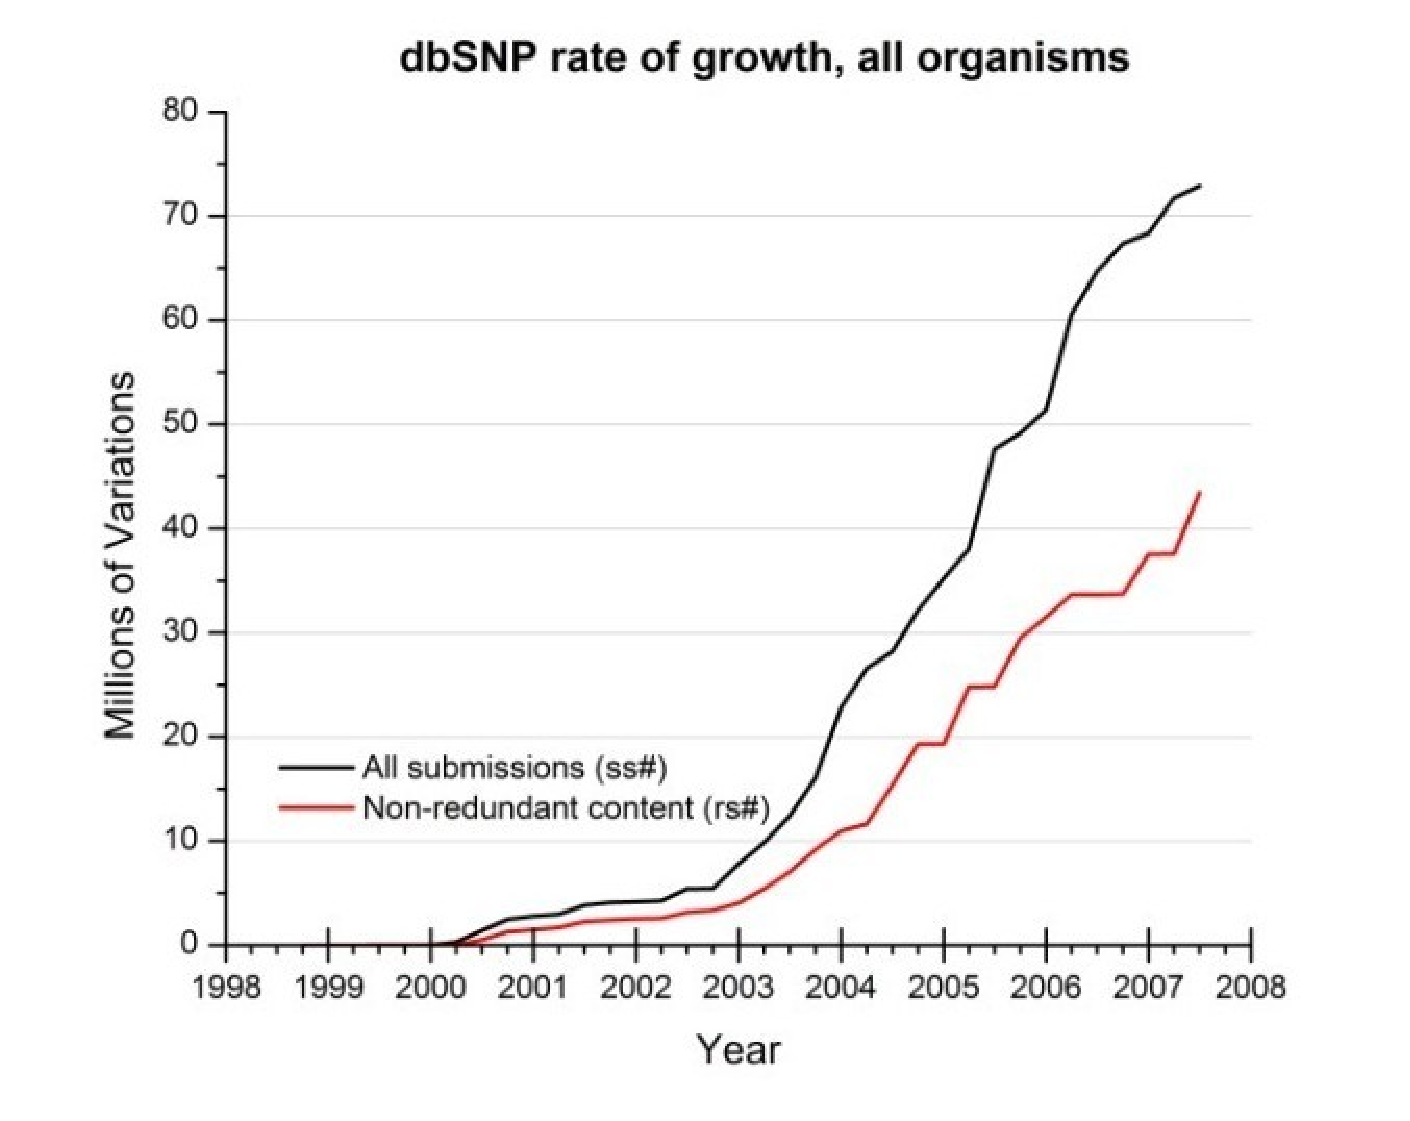
\includegraphics[width=\linewidth]{documents/latex/figures/1/increase_dbsnp.pdf}
\caption{Crecimiento de la base dbSNP a partir del Proyecto Genoma Humano (NCBI-NIH, 2008). La curva negra corresponde a todos los SNPs subidos a la base y la curva roja a los clusters de SNPs que referencian a la misma posición del genoma.}
\label{fig:dbsnp_growth_rate}
\end{minipage}%
\end{figure}

\textbf{El problema biológico que intentaremos atacar es poder predecir aquellos SNPs missense no investigados aún cuyo cambio en el aminoácido de la proteína generada pueda estar asociado a alguna patogénesis}. 

\section{Enfoque computacional}

Para abordar este problema, decidimos usar métodos de aprendizaje automático. El aprendizaje automático es un método computacional (dentro del área de la inteligencia artificial y la estadística) que consiste en aprender a partir de los datos. 

Existen diferentes formas de categorizar los algoritmos de aprendizaje automático. De acuerdo a Barber \cite{Barber2011}, una de las formas posibles es la categorización de acuerdo a la cantidad de tipo de supervisión durante la fase de entrenamiento. Este aprendizaje puede ser:

\begin{itemize}
\item Supervisado, en donde se utilizan ejemplos previos que están ``rotulados'', es decir que poseen una variable de respuesta conocida y se busca conseguir una predicción lo más certera posible sobre nuevos datos. Esta variable de respuesta puede ser continua (problema de regresión) o dividida en clases (problema de clasificación). 
\item No supervisado, donde el objetivo es encontrar distintos grupos o clusters dentro de los datos.
\item Semi-supervisado, en el que se trabaja con un pequeño conjunto de datos etiquetados y un conjunto mucho mayor de datos no etiquetados. El objetivo consiste en usar este último conjunto para mejorar el clasificador construido con los datos etiquetados.
\item Por refuerzo, donde un \textit{agente} observa el entorno y realiza diferentes acciones para maximizar la recompensa. El modelo a aprender entonces es la estrategia que le permite tomar decisiones ante determinadas situaciones. 
\end{itemize}

Durante la fase de entrenamiento estos algoritmos ajustan sus parámetros de acuerdo a los datos recibidos. En la mayoría de los casos estos algoritmos también poseen hiperparámetros, que no se modifican durante la fase de entrenamiento y determinan algunas de sus características. Estos hiperparámetros pueden ser optimizados mediante técnicas de validación cruzada (ver sección \ref{pipeline}). 

La creciente producción de trabajos nos aporta una gran cantidad de efectos conocidos de las variantes proteicas, y a su vez la ubicación (\textit{locus}) del SNP \textit{missense} responsable en el genoma. Estos datos se encuentran (en gran parte) de forma abierta y gratuita, lo que nos permite aplicar este enfoque computacional. Usando esta fuente de datos entrenaremos un modelo (de forma supervisada) que pueda predecir con un cierto grado de precisión el efecto de una variante aún no reportada. 

% \newpage

\subsection{Aprendizaje supervisado}

Como mencionamos anteriormente, el aprendizaje supervisado trata de predecir una respuesta usando un modelo generado con datos correctamente etiquetados. Definido de manera formal, dado un set de datos $ \mathcal{D} = \{(x^n, y^n), n = 1...N\}$  buscamos aprender la relación entre el ejemplo $x$ y la variable de respuesta $y$ tal que al recibir un nuevo ejemplo $x^*$ la respuesta predicha $y^*$ sea precisa \cite{Barber2011}. La precisión está definida formalmente por la función de pérdida o \textit{Loss Function}, $L(y^{pred}, y^{true})$. Esta función nos permite medir el costo de errar en la predicción y por lo tanto entrenar nuestro modelo de manera que el valor de la función de pérdida usando los datos de entrenamiento sea mínimo o cercano al mínimo.

En el contexto de nuestro problema, cada vector $x$ del set de datos $\mathcal{D}$ es un conjunto de variables que describen a distintos niveles (estructural, físico-químico, genómico) al SNP y a su variante proteica producida e $y$ es el efecto producido en el organismo, basándonos en reportes de Humsavar y Clinvar. Al ser una variable de tipo binaria, podemos aplicar algoritmos de clasificación para este problema. Posteriormente en la secciones \ref{pipeline}, \ref{confusion_matrix} y \ref{eval_metrics} analizaremos el proceso general por el cuál estos algoritmos son entrenados y las métricas para evaluar su desempeño.

A continuación haremos un recorrido por los distintos métodos de clasificación que utilizaremos en esta tesis. Estos métodos se encuentran implementados en el módulo \texttt{scikit-learn} de Python \cite{scikit-learn}, excepto por el método Gradient Boosting y su implementación XGBoost \cite{xgboost}. En cada uno de los apartados mencionaremos su funcionamiento general, sus parámetros y sus hiperparámetros. Para estos últimos mencionaremos entre paréntesis su nombre usado en la implementación.

\subsubsection{Regresión logística}

La regresión logística (LR) es un modelo basado en la regresión lineal. Al igual que ésta, consiste en buscar los coeficientes de una función de manera que el valor de la función de pérdida sea el mínimo. A diferencia de la regresión lineal, que usa una función lineal (o polinomial) para aproximar los puntos (que son valores continuos), la regresión logística usa la función logística para aproximar los valores (que son categóricos). Esta función, generalizada para múltiples variables predictoras y variable de respuesta binaria se define como:

\begin{equation*}
h_{\theta}(\boldsymbol{X}) = \frac{1}{1 + e^{\theta^{T}\boldsymbol{X}}} = Pr(Y = 1 | \boldsymbol{X}; \theta)
\end{equation*}

donde $\boldsymbol{X}$ representa el vector de variables predictoras, $\theta$ es el vector de coeficientes ($\theta^{T}$ representa al vector transpuesto) e $Y$ es la variable de respuesta \cite{Barber2011}. Lo que se busca modelar, es la probabilidad de pertenecer a una clase determinada (simbolizada con '1'), cuando las variables observadas son $\boldsymbol{X}$ y usando los parámetros $\theta$. La probabilidad de pertenecer a la otra clase entonces, es igual a 1 - $h_{\theta}(\boldsymbol{X})$. 

Los parámetros $\theta$ son obtenidos buscando maximizar la verosimilitud con los parámetros de la distribución real de los datos \cite{Hastie2001}, mientras que los hiperparámetros ($\Tilde{\theta}$) se obtienen usando validación cruzada (ver sección \ref{pipeline}). Los hiperparámetros que buscaremos optimizar son dos:

\begin{itemize}
    \item El parámetro de regularización (\texttt{C}): Parámetro usado para penalizar el uso de muchas variables en la función de pérdida, simplificando el modelo y previniendo un posible \textit{overfitting}.
    \item El balance de las clases (\texttt{class\_weight}): Pesos asociados a la importancia a la que se le da reconocer una determinada clase, penalizando el error en la función de pérdida con un valor asignado en lugar de 1. 
\end{itemize}

\subsubsection{Support Vector Machines}

Las Support Vector Machines (SVM) se desarrollaron inicialmente como métodos lineales de clasificación, al igual que la regresión logística. Esto significa que también buscan una frontera de decisión (\textit{decision boundary}) que define la clase a la que pertenecen los datos usando una combinación lineal de las variables predictoras. En este caso no se busca hallar los parámetros de la distribución a modelar sino que el objetivo reside en encontrar el hiperplano (\textit{Support Vector}) que mejor separe a los datos de entrenamiento \cite{Hastie2001}. Posteriormente este método fue extendido para buscar un hiperplano en un espacio de variables transformado (método no lineal). Esta transformación se logra reemplazando el producto interno por una función kernel. En este trabajo haremos uso de la función de base radial (RBF, por sus siglas en inglés), que es la más comúnmente usada en este método. En este algoritmo buscaremos optimizar dos hiperparámetros: 

\begin{itemize}
    \item El parámetro de penalidad (\texttt{C}): Este parámetro regula que tan bien debe el hiperplano separar las clases a costa de una distancia menor en la frontera de decisión. Es decir, un valor elevado de \texttt{C} se ajustará mejor a los datos de entrenamiento, mientras que un valor bajo será más general, a costa de errores.
    \item Gamma (\texttt{gamma}): Define que tan lejos alcanza la influencia de cada uno de los ejemplos de entrenamiento en la creación de la frontera de decisión.  
\end{itemize}  

\subsubsection{Random Forest}

A diferencia de los algoritmos anteriores, Random Forest (RF) esta basado en un método de clasificación basado en árboles de decisión. Estos métodos se caracterizan por segmentar el espacio de predicción en un número de regiones. Para entender Random Forest, resulta muy útil conocer el funcionamiento de éstos árboles. 

Un árbol de decisión se construye dividiendo el espacio de variables de forma recursiva, recorriendo la lista de variables y seleccionando la variable que mejor divide las clases de acuerdo a un criterio determinado. El criterio que decidimos usar en este trabajo, por ser el más usado en tareas de clasificación, es el índice Gini (también referido como pureza):

\begin{equation*}
    G = \sum_{k = 1}^{K} \hat{p}_{mk}(1 - \hat{p}_{mk})
\end{equation*}

donde $\hat{p}_{mk}$ representa la proporción de la clase $k$ en la región $m$ \cite{Hastie2001}. Uno de los principales problemas que presenta este enfoque es la alta varianza (\textit{variance}) con respecto a los datos de entrenamiento. Si la profundidad del árbol es muy grande, aumenta el riesgo de \textit{overfitting} en los datos que poseemos. 

En el caso de Random Forest, se construyen distintos árboles de decisión con subconjuntos de variables escogidos de forma aleatoria, con el objetivo de disminuir la varianza. A la vez, al ser árboles de poca profundidad (que favorecen el \textit{underfitting}), se genera una cantidad alta de árboles para solucionar el problema de alto sesgo (\textit{bias}). 

Esta técnica consistente en combinar distintos algoritmos para obtener un mejor predictor se la denomina \textit{ensamble}, y en particular, Random Forest se enmarca dentro de la técnica de \textit{bagging}. Esto significa que la predicción final se obtiene a través de un promedio de los predictores que componen el método con igual peso.

Una de las principales ventajas de Random Forest es su interpretabilidad. Esto se expresa en la posibilidad de calcular fácilmente la importancia de las variables en el modelo. La importancia de una variable (o \textit{feature importance}) se calcula como el promedio del índice Gini en cada uno de los nodos de los árboles donde aparece, expresada proporcionalmente a la importancia máxima de todas las variables \cite{Hastie2001}.
Finalmente, el algoritmos posee una serie de hiperparámetros a ser tuneados. Nosotros buscaremos optimizar los siguientes:

\begin{itemize}
    \item Profundidad del árbol (\texttt{max\_depth}): La profundidad máxima de cada árbol.
    \item Estimadores (\texttt{n\_estimators}): La cantidad de árboles.
    \item Cantidad de variables por árbol (\texttt{max\_features}): En cada split del árbol, se puede fijar la cantidad de variables a comparar.
\end{itemize}

\subsubsection{Gradient Boosting y XGBoost}

Gradient Boosting (GB) es otro método de ensamble, que como las otras técnicas de \textit{boosting}, genera modelos de forma iterativa, modificando el algoritmo para intentar corregir los errores de la iteración anterior. Esta es una diferencia crucial con respecto a los algoritmos de \textit{bagging}, como Random Forest, que genera modelos de forma paralela. La forma en que Gradient Boosting busca mejorar iterativamente es modelando el vector residual (o en otras palabras, la distancia entre la predicción y la variable a predecir) generando de esta manera un modelo aditivo que se puede representar de la siguiente manera:

\begin{equation*}
    F_{m}(X) = F_{m - 1}(X) + \eta \cdot \Delta_{m}(X) 
\end{equation*}

donde $F_{m - 1}(X)$ es el modelo del paso anterior, $\Delta_{m}(X)$ es el modelo del vector residual y $\eta$ es el \textit{learning rate}, un hiperparámetro que busca regularizar la importancia de este factor en el modelo final para reducir el \textit{overfitting} \cite{gradient}. 

En este trabajo vamos a utilizar XGBoost (XGB), una implementación de Gradient Boosting con árboles muy utilizado en competencias Kaggle \cite{xgboost}. Este algoritmo cuenta con una gran cantidad de hiperparámetros, al ser un método de ensamble combina los hiperparámetros de los \textit{tree boosters} con los pertenecientes al método Gradient Boosting. Decidimos limitarnos a un número relativamente pequeño de hiperparámetros buscando referencias de su uso, aunque dejamos la exploración de los restantes para un trabajo futuro. Los hiperparámetros explorados fueron:

\begin{itemize}
    \item Peso mínimo de las hojas (\texttt{min\_child\_weight}): Mínima suma del peso de las instancias (hessiano) necesaria en un hoja para dejar de realizar cortes.
    \item Gamma (\texttt{gamma}): Mínima pérdida requerida para la creación de un nuevo corte en el árbol.
    \item Muestreo (\texttt{subsample}): Proporción de muestra de los ejemplos antes de la construcción del árbol. 
    \item Cantidad de variables por árbol (\texttt{colsample\_bytree}): Mismo parámetro que en Random Forest.
    \item Profundidad máxima (\texttt{max\_depth}): Mismo parámetro que en Random Forest.
\end{itemize}

\subsection{Pipeline de entrenamiento, validación y evaluación} \label{pipeline}

Cada uno de estos métodos involucran una fase de entrenamiento, validación y evaluación. En la fase de entrenamiento los algoritmos ajustan sus datos de acuerdo a sus distintas funciones de pérdida. En nuestro trabajo también buscamos aproximarnos al mejor set de valores de hiperparámetros usando una técnica llamada \textit{Grid-Search}. Este método consiste en evaluar distintos valores para cada parámetro, que en conjunto forman una grilla (o \textit{grid}). 

Para cada conjunto de hiperparámetros de esta grilla se entrena el modelo y finalmente se elige el conjunto de hiperparámetros que haya tenido mejor performance (bajo alguna métrica, ver sección \ref{eval_metrics}). Al evaluar la performance de cada conjunto de hiperparámetros no podemos volver a usar el mismo conjunto de datos para el que fue entrenado, por lo que para evitar esto usamos otra técnica llamada \textit{k-fold Cross Validation}. La idea es generar un corte (\textit{split}) en el dataset de entrenamiento con el objetivo de poder evaluar los hiperparámetros en un conjunto de datos que no haya sido utilizado (conjunto de validación). Este procedimiento se realiza $k$ veces con diferentes splits realizados al azar, con una proporción igual en cada subconjunto o \textit{fold}. Estos \textit{folds} son disjuntos entre sí. Una vez elegido el modelo entrenado con el mejor conjunto de hiperparámetros se evalúa en un dataset de evaluación (que no fue usado durante el entrenamiento) de acuerdo a las métricas de la sección \ref{eval_metrics}.

\newpage

\subsection{Matriz de confusión} \label{confusion_matrix}

Una matriz de confusión en el caso de un problema de clasificación binario es una tabla de contingencia con cuatro posibles resultados, como podemos ver en la figura \ref{fig:confusion_matrix}. Dado un clasificador y un conjunto de instancias del que conocemos sus clases, esta tabla informa de la cantidad de instancias correctamente clasificadas como positivas (verdaderos positivos) y la cantidad de instancias correctamente clasificadas como negativas (verdaderos negativos). También, si el valor predicho es negativo y la clase verdadera es negativa es un verdadero negativo, en caso contrario es un falso negativo \cite{Fawcett2006}. Esta tabla puede expresarse en valores absolutos o relativos a la cantidad total de instancias. A partir de estos conjuntos (VP, VN, FP y FN) calculamos las métricas con las que evaluamos el modelo, descriptas a continuación.

\begin{figure}[H]
    \centering
    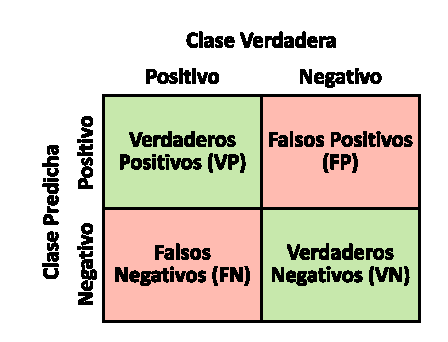
\includegraphics[scale=1]{documents/latex/figures/1/confusion_matrix.pdf}
    \caption{La matriz de confusión y sus cuatro posibles casos: Verdaderos positivos, verdaderos negativos (marcados en verde), falsos positivos y falsos negativos (marcados en rojo).}
    \label{fig:confusion_matrix}
\end{figure}


% \newpage

\subsection{Métricas de evaluación} \label{eval_metrics}

Las medidas que utilizaremos para evaluar la performance del modelo son las siguientes:

\begin{itemize}

    \item \textbf{Precisión}: La Precisión del modelo, está medida como la cantidad de positivos correctamente clasificados (VP) sobre la cantidad de instancias clasificadas como positivas: verdaderos positivos (VP) y falsos positivos (FP).
    
    \begin{equation*}
        \frac{VP}{VP + FP}
    \end{equation*}
    
% \pagebreak
    \item \textbf{Sensibilidad o Recall}: La Sensibilidad (o \textit{Recall}, en inglés), corresponde a la cantidad de verdaderos positivos sobre el total de positivos: verdaderos positivos (VP) y falsos negativos (FN).
    
    \begin{equation*}
        \frac{VP}{VP + FN}
    \end{equation*}

    \newpage
    
    \item \textbf{F1-Score}: El F1-Score es el promedio armónico entre la Precisión y el Recall. Usamos el promedio armónico de manera de afectar negativamente el resultado si alguno de los valores es especialmente bajo. Posee un rango de 0 a 1. 
    
    \begin{equation*}
        F_1 = \frac{2}{\tfrac{1}{\mathrm{recall}} + \tfrac{1}{\mathrm{precision}}} = 2 \cdot \frac{\mathrm{precision} \cdot \mathrm{recall}}{\mathrm{precision} + \mathrm{recall}}
    \end{equation*}
    
    % \newpage
    
    \item \textbf{Área bajo la curva ROC (AUC)}: La curva ROC está generada por dos métricas principales, FPR y TPR:
    
    \begin{multicols}{2}
        \begin{equation*}
        TPR = \frac{VP}{VP + FN}
        \end{equation*}
        \break
        \begin{equation*}
        FPR = \frac{FP}{FP + VN} 
        \end{equation*}
    \end{multicols}
    
    En un contexto de clasificación binaria, si ordenamos al score de predicción final de mayor a menor y consideramos positivos a todos aquellos a la izquierda del umbral de decisión (\textit{threshold}), obtendremos una tasa de verdaderos positivos y de falsos positivos (TPR y FPR respectivamente). Esto puede verse en la figura \ref{fig:threshold_auc}.
    
    \begin{figure}[H]
    \centering
        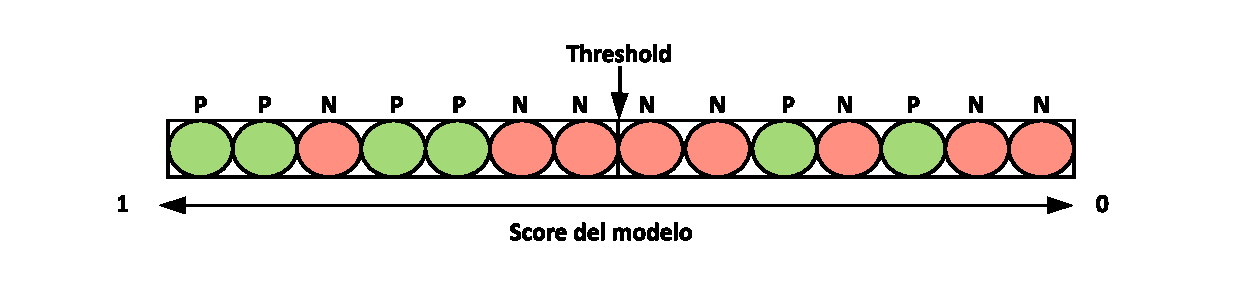
\includegraphics[scale=0.8]{documents/latex/figures/1/threshold_auc.pdf}
    \caption{Predicciones ordenadas de mayor a menor, donde el \textit{threshold} asigna clasificación positiva y negativa. El color de las instancias indica el valor real. En este caso el $TPR$ es igual a $2/3$ y el FPR es igual a $3/8$.}
    \label{fig:threshold_auc}
    \end{figure}
    
    La curva característica operativa del receptor (ROC, por sus siglas en inglés) es la representación gráfica de la relación entre el FPR y el TPR al mover el umbral de decisión. 

    En la figura \ref{fig:example_roc} puede verse la curva que representa el ejemplo de la figura \ref{fig:threshold_auc}.
    
    \begin{figure}[H]
        \centering
        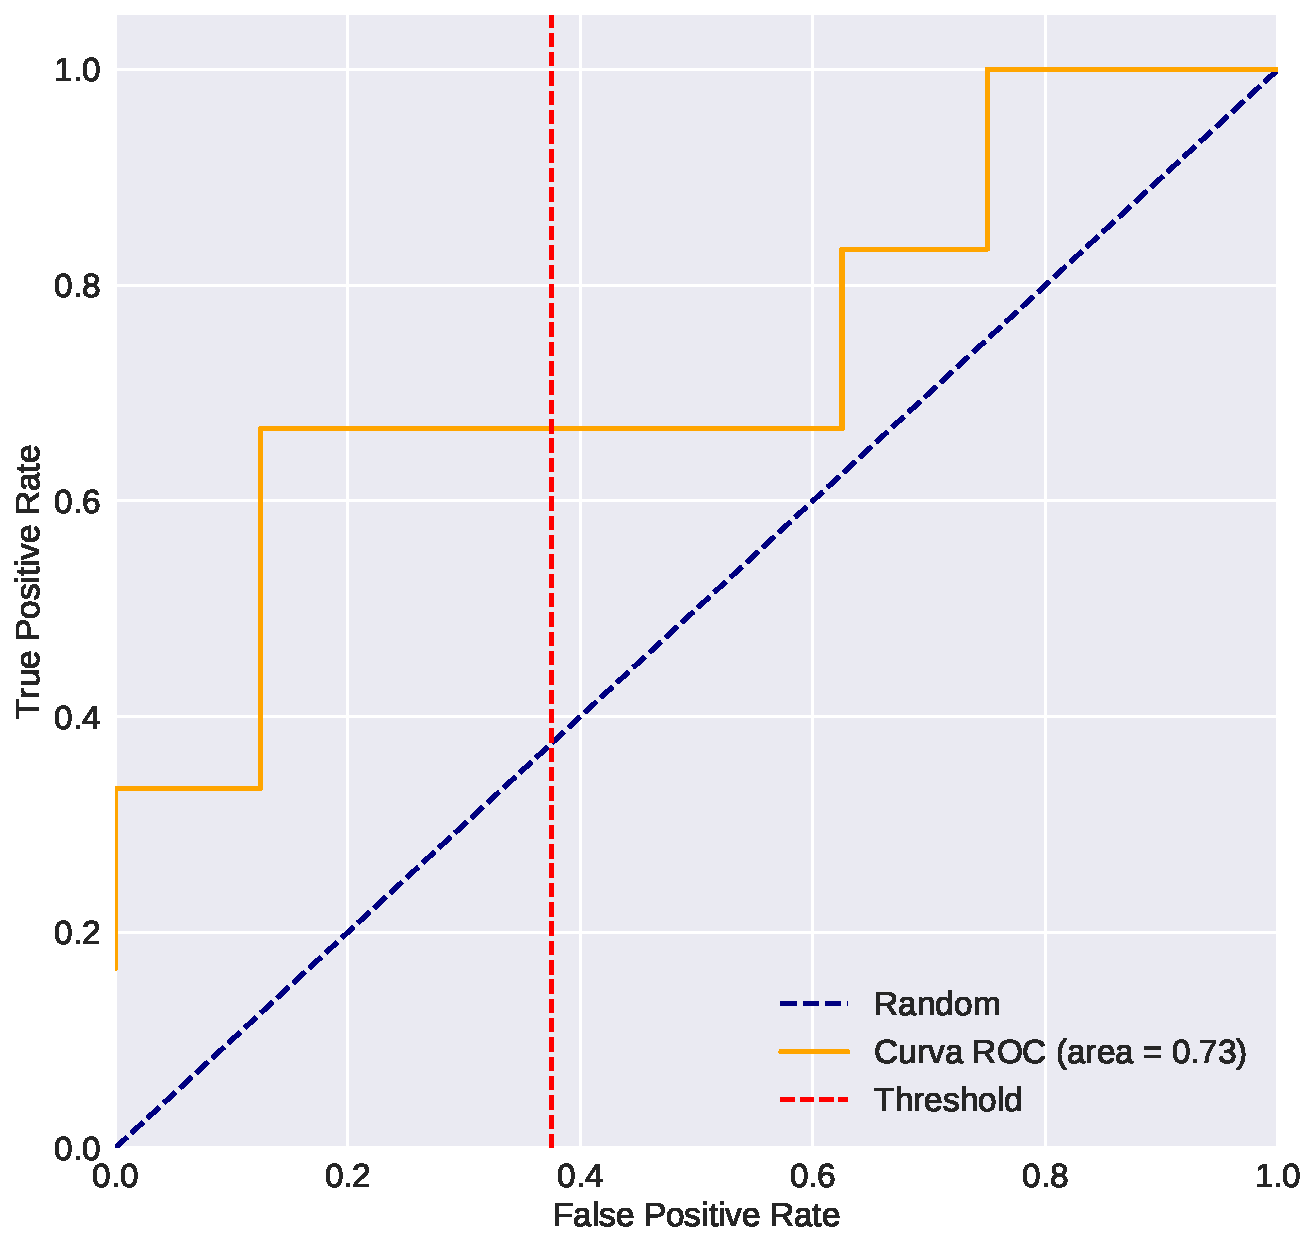
\includegraphics[scale=0.35]{documents/latex/figures/1/roc_ejemplo.pdf}
        \caption{Curva ROC de la clasificación de la figura \ref{fig:threshold_auc}. La línea punteada roja representa el umbral de decisión, que fijó el FPR y TPR en los valores anteriormente mencionados.}
        \label{fig:example_roc}
    \end{figure}
    
    Su área (AUC, por sus siglas en inglés) equivale a la probabilidad de que el modelo clasifique una instancia positiva cualquiera ``mejor'' que una instancia negativa cualquiera (estadístico Mann-Whitney $U$ \cite{doi:10.1256/003590002320603584}). Dadas dos muestras de tamaño $n_1$ y $n_2$, el estadístico Mann-Whitney $U$ se define como:
    
    \begin{equation*}
        U = \sum_{i = 1}^{n_1} r_{1i} - \frac{n_1 (n_1 + 1)}{2}
    \end{equation*}
    
    donde $r_{1i}$ es el ranking del elemento $i$ de la muestra $n_1$. La equivalencia con este estadístico viene de considerar a los verdaderos positivos y falsos positivos como muestras $n_1$ y $n_2$ respectivamente. Su distribución es aproximadamente normal para muestras grandes \cite{mann1947}, lo que nos permite calcular su intervalo de confianza. Otro método, el test de DeLong, utiliza este mismo concepto para evaluar y comparar curvas de AUC \cite{DeLong}.

\end{itemize}

% \newpage


\section{Trabajos relacionados}

A partir de mutaciones conocidas y sus propiedades asociadas, deseamos explorar un método de aprendizaje automático supervisado que nos permita generar un modelo que, ante una mutación no estudiada, pueda predecir su patogenicidad. Para recolectar datos, asociados a mutaciones conocidas, existen múltiples herramientas. En particular, para el presente trabajo vamos a explorar: VarQ, VEST y FATHMM-MKL.

\subsubsection{VarQ}

VarQ es una herramienta generada en la BIA (Plataforma Bioinformática Argentina) por Leandro Radusky \cite{Radusky2017}. Esta herramienta permite extraer datos estructurales de variantes proteicas de un sólo aminoácido (SAS, por sus siglas en inglés) tomando información de diferentes bases de datos o aplicaciones (PDB, PFam, 3DID, entre otras), permitiendo el análisis manual de los diferentes cambios estructurales, como el tipo de actividad, el plegamiento, si pertenece a un sitio activo, o si forma parte en interfaces proteína-proteína, como se ve en la figura \ref{fig:varq_pipeline}. 

\begin{figure}[H]
    \centering
    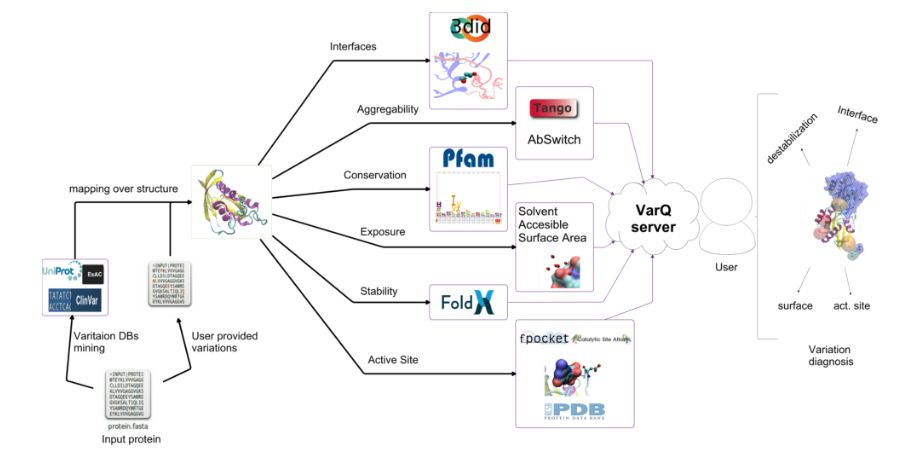
\includegraphics[scale=0.45]{documents/latex/figures/1/pipeline.png}
    \caption{Pipeline de extracción de datos de la herramienta VarQ. Esta figura fue extraída de la tesis de doctorado de Leandro Radusky \cite{Radusky2017}.}
    \label{fig:varq_pipeline}
\end{figure}

En la primera parte de esta tesis hacemos uso del trabajo de tesis de grado de Santiago Moreno (todavía en elaboración). Uno de sus objetivos principales fue generar un dataset de variantes a nivel de proteínas (al que denominaremos dataset VarQ), y evaluar la performance de un modelo que predice el efecto de la mutación usando las variables que provee esta herramienta. En la capítulo \ref{ch:desarrollo_varq} presentaremos un modelo de clasificación, variando las técnicas de aprendizaje automático presentadas, y creado en base a las variables que provee a este dataset. Posteriormente encontraremos sus limitaciones para tal fin.

\subsubsection{VEST}

VEST (\textit{Variant Effect Scoring Tool}) \cite{Carter2013} es un predictor de efectos funcionales de SNPs \textit{missense} desarrollado en el Karchin Lab de la Universidad de Johns Hopkins. Con esta herramienta (basada en Random Forest) analizaron aproximadamente 80,000 variantes anotadas de HGMD (\textit{Human Gene Mutation Database}) con variables de tipo genómicas, estructurales y físico-químicas usando la base de datos SNVBVox, desarrollado por el mismo equipo. A lo largo de nuestro trabajo integraremos muchas de las variables de esta base de datos a nuestros datasets.

\subsubsection{FATHMM-MKL}

FATHMM-MKL (\textit{Functional Analysis through Hidden Markov Models}) \cite{Shihab2015} es también un predictor de efectos funcionales de SNPs \textit{missense}, en regiones codificantes y no codificantes. El modelo está basado en SVM usando una combinación de múltiples kernels (\textit{Multiple Kernel Learning, MKL}). Fue desarrollado en la Universidad de Bristol. Uno de los puntos interestantes del trabajo es un suplemento con la descripción de las variables usadas. A partir de este informe buscaremos conseguir algunas de las variables usadas que hayan tenido mayor impacto en el modelo.

% \newpage


\section{Objetivos y estructura del trabajo}

El objetivo del trabajo se centra en responder una serie de interrogantes generados a partir del estudio de los trabajos previos:

\begin{itemize}
    \item El dataset de VarQ se compone esencialmente de variables de tipo estructural. ¿Es posible enriquecerlo con variables de otras dimensiones (físico-químicas, genómicas, filogenéticas)?
    \item ¿Cómo afectan las distintas variables a nuestros modelos de predicción de patogenicidad de los SNPs? ¿Cuáles son las más importantes para predecir una variante patogénica?
    \item ¿Cuáles son los mejores algoritmos de aprendizaje automático para resolver este tipo de problemas y cuáles son sus hiperparámetros?
    
\end{itemize}

Estos puntos serán abordados generando y estudiando modelos de aprendizaje automático sobre distintos conjuntos de variables descriptivas para los SNPs, como se describe a continuación:

\begin{itemize}
    \item Modelo usando el dataset VarQ
    \item Modelo usando propiedades físico-químicas de la proteína
    \item Modelo usando variables genómicas
    \item Integración de propiedades físico-químicas y variables genómicas
    \item Integración de propiedades físico-químicas, variables genómicas y las variables del dataset VarQ.
\end{itemize}


